\documentclass{article}

\usepackage[letterpaper]{geometry}
\usepackage{amsmath}
\usepackage{siunitx}
\usepackage{graphicx}

\title{4261 HW 7}
\author{Duncan Wilkie}
\date{}

\begin{document}

\maketitle

\section{}
In the tight-binding and nearly-free electron models, one observes discontinuities in the dispersion plot at the Brillouin zone boundaries.
Connected components of the dispersion plot are called bands.
Sodium is in group I, and as such has a half-filled valence band, making it a metal, because if a Coulomb potential is applied, the electron
from one atom is free to move to the opposite-spin state in the other half of the valence band on its neighbor, i.e. it's conductive.
Calcium, in group II, has valence 2, so one might think it's an insulator.
However, it is possible for the potential to be such that the band energies overlap, and one electron half-fills the valence band
while the other goes into the conduction band.
Evidently, this occurs for calcium.
Carbon, silicon, and germanium are all group IV, and so one would expect the valence electrons to form two completely filled bands.
Indeed this is the case; it just so happens that the band gaps in silicon and germanium are sufficiently smaller than diamond to make
the latter an insulator and the others semiconductors.
Diamond is transparent because its insulating nature means that incident light cannot excite the electrons unless the photons are
sufficiently energetic to move them to the conduction band.
It so happens that diamond's band gap is sufficiently large that the excitation frequencies are higher than those of visible light, so
visible light doesn't interact with the atoms in the crystal, and it is transparent.

A sketch of the given dispersion in the extended zone scheme with $k_{x}=k_{y}$ appears below.
\[
  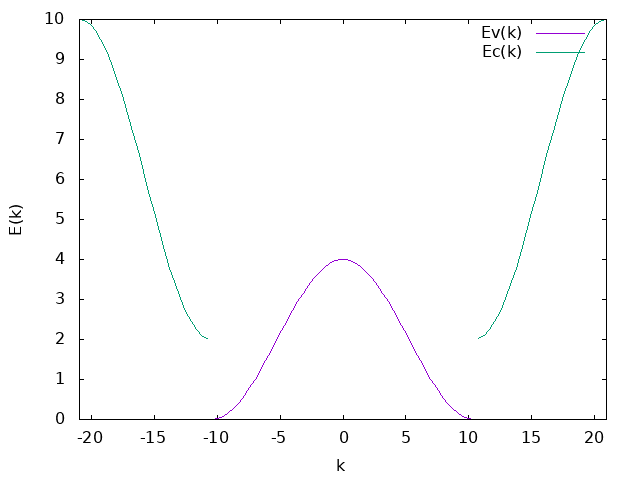
\includegraphics[scale=.8]{plot1.png}
\]
The band gap clearly occurs at the Brillouin zone boundary, in this case $\pm \pi/0.3$, and has magnitude
\[
  \epsilon_{c}(0)-\epsilon_{v}(\pi/0.3)=\SI{2}{eV}-\SI{0}{eV}=\SI{2}{eV}
\]
Near the band edges, we may approximate $\cos(k_{x}a)\approx 1-k_{x}^{2}a^{2}/2$ and $\cos(k_{y}a)\approx 1-k_{y}^{2}a^{2}/2$ to get
\[
  \epsilon_{c}(\vec{k})=c\Rightarrow 6-2(1-k_{x}^{2}a^{2}/2+1-k_{y}^{2}a^{2}/2)=c
  \Rightarrow k_{x}^{2}+k_{y}^{2}=c_{1}^{2}
\]
and
\[
  \epsilon_{v}(\vec{k})=c \Rightarrow 2+(1-k_{x}^{2}a^{2}/2+1-k_{y}^{2}a^{2}/2)
  \Rightarrow k_{x}^{2}+k_{y}^{2}= c_{2}^{2}
\]
which are the equations for $k$-space circles.
In the language of the effective mass section, we have $\alpha=a^{2}/2$ (using the expansion of cosine about its minimum) from which we can find the effective mass via
\[
  \frac{\hbar^{2}}{m^{*}}=2\alpha
  \Leftrightarrow m^{*}=\frac{\hbar^{2}}{2(a^{2}/2)}=\frac{\hbar^{2}}{a^{2}}
  =\frac{(\SI{1.05e-34}{J\cdot s})^{2}}{(\SI{0.3}{nm})^{2}}
  =\SI{1.23e-49}{kg}
\]
The effective mass of the holes is equal to this (since the expansion of cosine about its maximum and minimum have the same second term
have the same magnitude, but different sign; the term is negated in the computation of $m^{*}$).
Using the expressions derived in the book,
\[
  g_{c}(\epsilon\geq \epsilon_{c})=\frac{(2m_{e}^{*})^{3/2}}{2\pi^{2}\hbar^{3}}\sqrt{\epsilon-\epsilon_{cz}}
\]
and
\[
  g_{v}(\epsilon\leq \epsilon_{v})=\frac{(2m_{h}^{*})^{3/2}}{2\pi^{2}\hbar^{3}}\sqrt{\epsilon_{v}-\epsilon}
\]
Plotting these,
\[
  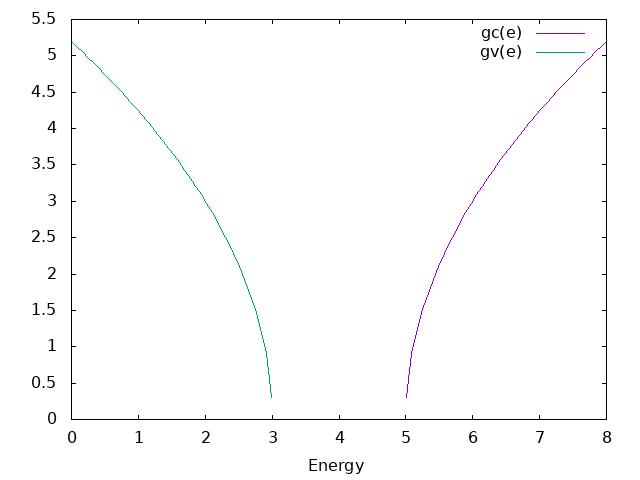
\includegraphics[scale=0.8]{plot2.png}
\]
The given energies are two solutions for a tight binding model with one site per atom on a two-dimensional square lattice with different
site energies but the same hopping term; the general form of such a solution is
\[
  E(\vec{k})=\epsilon_{0}-2t\cos(k_{x}a)-2t\cos(k_{y}a)
\]
\section{}
When $k_{B}T\ll \epsilon_{g} $, there are very few electrons in the conduction band, so the system is well-described by Boltzmann statistics.
The occupancy of the conduction band is then given by
\[
  n(T)=\int_{\epsilon_{c}}^{\infty}g_{c}(\epsilon)\overline{n}_{F}(\epsilon)d\epsilon
  \approx \int_{\epsilon_{c}}^{\infty}\frac{(2m_{e}^{*})^{3/2}}{2\pi^{2}\hbar^{3}}\sqrt{\epsilon-\epsilon_{c}}e^{-\beta(\epsilon-\mu)}
\]
where the density of states is simply the Fermi gas density of states with zero at $\epsilon=\epsilon_{c}$ instead of $\epsilon=0$.
Making the change of variables to $x=\epsilon-\epsilon_{c}$, in which case $e^{-\beta(\epsilon-\mu)}=e^{-\beta x}e^{-\beta(\epsilon_{c}-\mu)}$,
\[
  =\frac{(2m_{e}^{*})^{3/2}}{2\pi^{2}\hbar^{3}}e^{-\beta(\epsilon_{c}-\mu)}\int_{0}^{\infty}\sqrt{x}e^{-\beta x}dx
\]
This integral evaluates to $\frac{1}{2}\beta^{-3/2}\sqrt{\pi}$, so the final result for electron occupancy is
\[
  n(T)=\frac{1}{4}\left( \frac{{2m_{3}^{*}}}{\pi \hbar^{2}} \right)^{3/2}e^{-\beta(\epsilon_{c}-\mu)}
\]
In the case of the hole occupation, all that changes is the $\sqrt{\epsilon_{c}-\epsilon}$ term in the density of states becomes
$\sqrt{\epsilon-\epsilon_{v}}$, which merely turns the argument of the exponential term in the final result to $-\beta(\mu-\epsilon_{v})$.
Writing it out,
\[
  p(T)=\frac{1}{4}\left( \frac{2m_{h}^{*}}{\pi\hbar^{2}} \right)^{3/2}e^{-\beta(\mu-\epsilon_{v})}
\]
The product of these is the law of mass action:
\[
  n(T)p(T)=\frac{1}{2}\left( \frac{k_{B}T}{\pi\hbar^{2}} \right)^{3}(m_{e}^{*}m_{h}^{*})^{3/2}e^{-\beta(\epsilon_{c}-\epsilon_{v})}
\]
which depends only on the effective masses and the band gap.
For an intrinsic material,
\[
  n=p=\sqrt{np}=\frac{1}{\sqrt{2}}\left( \frac{k_{B}T}{\pi\hbar^{2}} \right)^{3/2}(m_{e}^{*}m_{h}^{*})^{3/4}e^{-\beta E_{gap}/2}
\]
Evaluating this for the given band gap and electron/hole mass for silicon at room temperature,
\[
  n=\frac{1}{\sqrt{2}}\left( \frac{(\SI{1.38e-23}{J/K})(\SI{300}{K})}{\pi(\SI{1.05e-34}{J\cdot s})^{2}} \right)^{3/2}
  [\frac{1}{2}(\SI{9.11e-31}{kg})\frac{1}{2}(\SI{9.11e-31}{kg})]^{3/4}
\]
\[
  \cdot e^{-(\SI{1.1}{eV})(\SI{1.6e-19}{J/eV})/(\SI{1.38e-23}{J/K})(\SI{300}{K})}
\]
\[
  =\SI{3.10e6}{m^{-3}}
\]
For germanium, an identical calculation is possible:
\[
  n=\frac{1}{\sqrt{2}}\left( \frac{(\SI{1.38e-23}{J/K})(\SI{300}{K})}{\pi(\SI{1.05e-34}{J\cdot s})^{2}} \right)^{3/2}
  [\frac{1}{2}(\SI{9.11e-31}{kg})\frac{1}{2}(\SI{9.11e-31}{kg})]^{3/4}
\]
\[
  \cdot e^{-(\SI{0.75}{eV})(\SI{1.6e-19}{J/eV})/(\SI{1.38e-23}{J/K})(\SI{300}{K})}
\]
\[
  =\SI{3.28e12}{m^{-3}}
\]
When the dopant density is near the intrinsic undoped density calculated above, the intrinsic behavior is no longer valid.
From the given graph, it appears the concentration of donor ions is, reading the $y$-values for low $T$, roughly $\SI{2e19}{m^{-3}}$.
The band gap is, since it's a semilog plot, simply related to the slope at high temperature.
The slope appears to be around $\SI{-1500}{K}$, which yields from
\[
  \textrm{slope}=E_{g}/(2k_{B})\Rightarrow E_{g}=2(\SI{1.38e-23}{J/K})(\SI{1500}{K})=\SI{4.14e-20}{J}=\SI{0.26}{eV}
\]
The carrier density could be measured by detecting the Hall voltage, and could have experimental error due to resistive losses as the
Hall current propagates, associated heating of the semiconductor, and so on.

\section{}
A hole is a pseudoparticle corresponding to the absence of an electron in the valence band of a material, useful because often
the number of electrons is far more than the number of holes.
The effective mass is computed by (using $|\vec{k}|=k$)
\[
  \frac{\hbar^{2}}{m^{*}}=-\frac{\partial^{2}E}{\partial k^{2}}
  \Leftrightarrow m^{*}=-\frac{\hbar^{2}}{\partial^{2}E/\partial k^{2}}
  =\frac{\hbar^{2}}{\SI{2e-37}{}}
  =\SI{5.51e-32}{kg}
\]
The energy of the hole is the negative of the energy the electron had in the band, so
\[
  E_{hole}=10^{-37}|\vec{k}|^{2}=\SI{4e-21}{J}
\]
The momentum of the hole is the negative of the momentum the electron had in the band, so
\[
  \vec{p}_{hole}=-\hbar\vec{k}=(-\SI{2.1e-26}{kg\cdot m/s})\hat{x}
\]
The velocity of the hole is
\[
  \vec{v}_{hole}=\frac{\nabla_{\vec{k}_{hole}}E_{hole}}{\hbar}=\frac{2\times 10^{-37}|\vec{k}|\hat{k}}{\hbar}
  =(-\SI{3.81e5}{m/s})\hat{x}
\]
The current density is then
\[
  pe\vec{v}_{hole}=(\SI{e5}{m^{-3}})(\SI{1.6e-19}{C})(\SI{-3.81e5}{m/s})\hat{x}
  =(-\SI{6.1e-9}{A/m^{2}})\hat{x}
\]
Intrinsic semiconductors are characterized by $n=p$, so the ratio of the expressions for $p$ and $n$ is
\[
  1=\frac{\frac{1}{4}\left( \frac{2m_{e}^{*}k_{B}T}{\pi\hbar^{2}} \right)^{3/2}e^{-\beta(\epsilon_{c}-\mu)}}
  {\frac{1}{4}\left( \frac{2m_{h}^{*}k_{B}T}{\pi\hbar^{2}} \right)^{3/2}e^{-\beta(\mu-\epsilon_{v})}}
  =\left( \frac{m_{e}^{*}}{m_{h}^{*}} \right)^{3/2}e^{-\beta(\epsilon_{v}+\epsilon_{c}-2\mu)}
\]
\[
  \Leftrightarrow \frac{3}{2}\ln\left( \frac{m_{h}^{*}}{m_{e}^{*}} \right)=-\beta(\epsilon_{v}+\epsilon_{c})+2\beta\mu
  \Leftrightarrow \mu = \frac{\epsilon_{v}+\epsilon_{c}}{2}+\frac{3}{4}k_{B}T\ln\left( \frac{m_{h}^{*}}{m_{e}^{*}} \right)
\]
The limit as $T\to 0$ eliminates the second term, proving that $\mu$ is the average of $\epsilon_{c}$ and $\epsilon_{v}$
If the material is doped with donors, $n\geq p$, so the argument of the logarithm is multiplied by a constant greater than one.
If the dopant is an acceptor, this constant is less than one.
Factoring this constant out of the log, it is clear the chemical potential is larger than intrinsic in the case of donor doping,
and lower in the case of acceptor doping.
Using the result of problem 2, the undoped intrinsic carrier concentration is
\[
  p_{intrinsic}=\frac{1}{\sqrt{2}}\left( \frac{k_{B}T}{\pi\hbar^{2}}\right)^{3/2}(m_{e}^{*}m_{h}^{*})^{3/4}e^{-\beta E_{gap}/2}
\]
\[
  =\frac{1}{\sqrt{2}}\left( \frac{(\SI{1.38e-23}{J/K})(\SI{300}{K})}{\pi(\SI{1.05e-34}{J\cdot s})} \right)^{3/2}
  [(0.24)(\SI{9.11e-31}{kg})(0.4)(\SI{9.1e-31}{kg})]^{3/4}
\]
\[
  \cdot e^{-(\SI{1.6e-19}{J})/2(\SI{1.38e-23}{J/K})(\SI{300}{K})}
\]
\[
  =\SI{1.78e16}{m^{-3}}
\]
The given dopant concentration is much higher than this, we're in the extrinsic regime, and the material is $n$-doped.
Therefore, we can take the $n$ density to be simply the dopant concentration, yielding through the law of mass action's being the same
before and after the doping
\[
  n_{intrinsic}p_{intrinsic}=np\Rightarrow n_{intrinsic}^{2}=np\Leftrightarrow p=\frac{n_{intrinsic}^{2}}{n}=\frac{(\SI{1.78e16}{m^{-3}})^{2}}
  {(\SI{e23}{m^{-3}})}=\SI{3.17e9}{m^{-3}}
\]
\end{document}
%%% Local Variables:
%%% mode: latex
%%% TeX-master: t
%%% End:
